\documentclass[b5paper,11pt,fleqn,openright]{memoir}
\semiisopage[12]
\setlength{\uppermargin}{60pt}
\setlength{\headsep}{24pt}
\checkandfixthelayout[nearest]

\usepackage{cmbright}  % nice font

\usepackage[utf8]{inputenc}
\usepackage[hidelinks]{hyperref}
\usepackage{amsmath,amsfonts,amssymb,bm}%,amsthm}
\usepackage{gensymb}
\usepackage[capitalise]{cleveref}
\usepackage{graphicx,subcaption}
\usepackage{siunitx}
\usepackage{stmaryrd}
\usepackage{pgffor}
\usepackage{enumitem}
%\includeonly{mainmatter/uasstop.tex}
\usepackage[final]{pdfpages}

\usepackage{nomencl}
\makenomenclature

%float barrier
\usepackage{placeins}

\usepackage{lmodern}
\usepackage{algorithm}
\usepackage{algpseudocode}

% math stuff
\usepackage{cancel} 
\usepackage{bm}
\usepackage{upgreek}
\usepackage{amsmath}
\usepackage{amssymb}
\usepackage{relsize}
\usepackage{amssymb}




%pgf plot

\usepackage{pgfplots}
\pgfplotsset{compat=newest}
\usepackage{tikz}
\usetikzlibrary{plotmarks}
\usetikzlibrary{arrows.meta}
\usetikzlibrary{patterns}
\usetikzlibrary{patterns.meta} 
\usetikzlibrary{positioning}

\usepgfplotslibrary{patchplots}

\usetikzlibrary{external}
% \tikzexternalize % activate!
% \usetikzlibrary{shapes.geometric, arrows,positioning, calc, arrows.meta,scopes}
% and optionally (as of Pgfplots 1.3):

\pgfplotsset{plot coordinates/math parser=false}
\newlength\figureheight
\newlength\figurewidth 


\usepackage{multirow}
\usepackage{graphicx}
\usepackage{xcolor}

\usepgfplotslibrary{groupplots, external}

\definecolor{mycolor1}{rgb}{0.00000,0.44700,0.74100}%
\definecolor{mycolor2}{rgb}{0.85000,0.32500,0.09800}%
\definecolor{mycolor3}{rgb}{0.92900,0.69400,0.12500}%
\definecolor{mycolor4}{rgb}{0.46670,0.67450,0.18820}%
\definecolor{mycolor5}{rgb}{0.49400,0.18400,0.55600}%

\newlength{\twosubht}
\newsavebox{\twosubbox}


% definitions
\newcommand{\uniform}{$SG_U$}
\newcommand{\princ}{$SG_P$}
\newcommand{\userdefine}{$SG_A$}

\newcommand{\uniforms}{$SG_U$ }
\newcommand{\princs}{$SG_P$ }
\newcommand{\userdefines}{$SG_A$ }


\newlength{\imwidth}
\setlength{\imwidth}{14.cm}

\newlength{\imwidthmax}
\setlength{\imwidthmax}{15.cm}

%style=numeric-comp
\usepackage[natbib=true, style=numeric-comp, backend=biber, defernumbers, maxbibnames=99, maxcitenames=2, sorting=nyt, eprint=false, giveninits=true]{biblatex}
\addbibresource{ownPub/myownpubs.bib}
\addbibresource{bib.bib} 
\AtEveryBibitem{%
  % \clearfield{issn} % Remove issn
  \ifentrytype{online}{}{% Remove url except for @online
    \clearfield{url}
  }
}
\setlength\bibitemsep{1.5\itemsep}

% \definecolor{mylinkcolor}{rgb}{0.6745098039, 0.4196078431, 0.5921568627}%
\definecolor{mylinkcolor}{rgb}{0.,0.5019607843,0.6745098039}%
\definecolor{mycitecolor}{rgb}{0.9294117647, 0.4274509804, 0.4509803922}%
\definecolor{myurlcolor}{rgb}{0.4156862745, 0.6509803922, 0.6862745098}%


\hypersetup{
  linkcolor  = mylinkcolor,
  citecolor  = mylinkcolor,
  urlcolor   = mylinkcolor,
  colorlinks = true,
}



\DeclareFieldFormat{labelnumberwidth}{\mkbibbrackets{#1}}
\renewbibmacro*{cite}{%
  \printtext[bibhyperref]{%
    \printfield{labelprefix}%
    \ifkeyword{myPapers}
      {\printfield{labelnumber}}
      {\ifkeyword{myPapers2}
      {\printfield{labelnumber}}
      {\printfield{labelalpha}%
      \printfield{extraalpha}}}}}



\defbibenvironment{bibliographyNUM}
  {\list
     {\printtext[labelnumberwidth]{%
        \printfield{labelprefix}%
        \printfield{labelnumber}}}
     {\setlength{\labelwidth}{\labelnumberwidth}%
      \setlength{\leftmargin}{\labelwidth}%
      \setlength{\labelsep}{\biblabelsep}%
      \addtolength{\leftmargin}{\labelsep}%
      \setlength{\itemsep}{\bibitemsep}%
      \setlength{\parsep}{\bibparsep}}%
      \renewcommand*{\makelabel}[1]{\hss##1}}
  {\endlist}
  {\item}

\renewbibmacro{in:}{%
  \ifentrytype{article}{}{%
  \printtext{\bibstring{in}\intitlepunct}}}
  
 \preto\fullcite{\AtNextCite{\defcounter{maxnames}{99}}}
  
\newlength\drop
\makeatletter
\newcommand*\titleM{\begingroup% Misericords, T&H p 153
\setlength\drop{0.08\textheight}
\centering
\vspace*{\drop}
{\Huge\mdseries \thetitle }\\[\baselineskip]
%{\scshape the subtitle}\\[\baselineskip]
\vfill
{\large\mdseries \theauthor}\par
\vfill
{\mdseries Department of Civil and Mechanical Engineering\\Technical University of Denmark, 2800 Kongens Lyngby\\\@date}\par
\vspace*{0\drop}
\endgroup}
\makeatother


\newcommand{\diff}[2]{\frac{\partial #1}{\partial #2}}
\DeclareMathAlphabet{\mathpzc}{OT1}{pzc}{m}{it}
\usepackage{mathalpha}

\DeclareFontFamily{U}{mathx}{\hyphenchar\font45}
\DeclareFontShape{U}{mathx}{m}{n}{<-> mathx10}{}
\DeclareSymbolFont{mathx}{U}{mathx}{m}{n}
\DeclareMathAccent{\widebar}{0}{mathx}{"73}

%\chapterstyle{southall}


\makechapterstyle{southall-mod}{%
  \chapterstyle{default}
  \setlength{\afterchapskip}{1\baselineskip} %%%%%%%%% MOD: WAS 5\baselineskip
  \setlength{\beforechapskip}{18pt}%    \headindent %%%%%%% MOD: WAS 36pt
  \setlength{\midchapskip}{\textwidth}% \rightblock
  \addtolength{\midchapskip}{-\beforechapskip}
  \renewcommand*{\chapterheadstart}{}%\vspace*{0pt}} %%%% MOD: WAS 2\baselineskip
%%%  \renewcommand*{\chaptitlefont}{\huge\rmfamily\raggedright}
  \renewcommand*{\chaptitlefont}{\huge\rmfamily\memRTLraggedright}
  \renewcommand*{\chapnumfont}{\chaptitlefont}
  \renewcommand*{\printchaptername}{}
  \renewcommand*{\chapternamenum}{}
  \renewcommand*{\afterchapternum}{}
  \renewcommand*{\printchapternum}{%
    \begin{minipage}[t][\baselineskip][b]{\beforechapskip}
      {\vspace{0pt}\chapnumfont%%%\figureversion{lining}
                   \thechapter}
    \end{minipage}}
  \renewcommand*{\printchaptertitle}[1]{%
    \hfill\begin{minipage}[t]{\midchapskip}
      {\vspace{0pt}\chaptitlefont ##1\par}\end{minipage}}
  \renewcommand*{\afterchaptertitle}{%
    \par\vspace{\baselineskip}%
    \hrulefill \par\nobreak\noindent \vskip \afterchapskip}}

\newcommand{\InsertBlankPages}[1]{
  \foreach \blank in {1,...,#1} {
    \newpage
    \thispagestyle{plain}
    \mbox{}
  }%
}

\newlength{\commalabelwd}
\newcommand{\commalabel}[2]{%
  \settowidth\commalabelwd{\normalfont#2\hspace{\labelsep}}%
  \normalfont#2\ifdim#1<\commalabelwd\fi\hfill
}



% \chapterstyle{southall-mod}
% \chapterstyle{brotherton}
% \chapterstyle{madsen}
\chapterstyle{veelo}

\setcounter{tocdepth}{3}
\setsecnumdepth{subsection}


\title{Thesis Title}
\author{Ph.D. Candidate}
\date{Monnth Year}

\newcommand{\red}[1]{{\color{red}#1}}


\begin{document}


\frontmatter

\includepdf[pages=-,width=\paperwidth, templatesize={\paperwidth}{250mm}, offset=0 -0.2mm]{Cover/Front.pdf}
\cleardoublepage


\openany
\begin{titlingpage}
  \titleM
  \clearpage
  \noindent\textbf{Thesis title:} \\\noindent Thesis title
  \vspace{1.5em}

  \noindent\textbf{Author:}\\\noindent Ph.D. Candidate\\Department of Civil and Mechanical Engineering\\ Technical University of Denmark
  \vspace{0.5em}

  \noindent\textbf{Main Supervisor:}\\\noindent Main superviser\\Department of Civil and Mechanical Engineering\\ Technical University of Denmark
  \vspace{0.5em}

  \noindent\textbf{Co-supervisors:}\\
  \noindent Co-superviser\\Department of Civil and Mechanical Engineering\\ Technical University of Denmark
  \vspace{0.5em}

  \noindent\textbf{Funding and competing interests:}\\\noindent This work was funded by the Villum Foundation, through the Villum investigator project InnoTop. The author has no competing interests.
  \vspace{1.5em}

  \noindent\textbf{Duration:}\\\noindent The work has been carried out between the DATA0 and the DATA1.
  \vspace{2.2em}

  \noindent \copyright Ph.D. Candidate
  \vspace{1em}

  \noindent Department of Civil and Mechanical Engineering\\Technical University of Denmark\\ Nils Koppels Allé, Building 404 \\ DK-2800 Kongens Lyngby, Denmark
  \vspace{1em}

  \noindent MEK-PHD ISSN: \#\#\#\#-\#\#\#\#
\end{titlingpage}
\setcounter{page}{3}
\chapter*{Preface}

Bla bla bla...

\noindent Kongens Lyngby, \today,\\
\vspace{0.1cm}\\
\noindent \textit{Ph.D. Candidate}

\chapter*{Abstract}

Bla bla bla...

\chapter*{Resumé}

Bla bla bla...

\cleardoublepage
\chapter*{List of Publications}
\nocite{ownpub0,ownpub1}
\newrefcontext[sorting=none,labelprefix=P]
\printbibliography[env=bibliographyNUM,keyword=myPub,title={List of publications},heading=none,resetnumbers]
\newrefcontext[sorting=none,labelprefix=M]
\printbibliography[env=bibliographyNUM,keyword=myMan,heading=none,resetnumbers]
%https://tex.stackexchange.com/questions/553753/how-to-add-list-of-publication-in-thesis-class
%\endrefcontext

\cleardoublepage

{
  \hypersetup{linkcolor=black}
  \tableofcontents*
}



\mainmatter
\openright
\chapter{Introduction}

Bla bla bla...

Current state-of-the-art design approaches for photonic devices often rely on trial-and-error
experience-based multi-stage approaches using simplified physics models for individual
components. This may in part be due to the extensively developed and well-understood models
for the temporal and spatial confinement of light in pure photonic structures, such as photonic
crystals and waveguides, and in part due to the complexity of the full physics problems. Further, such design approaches often ignore multi-physics effects, such as . If these
effects are strong, and simultaneously have a large influence on the optical field, their omission in
the design process may lead to a suboptimal final device.

This Ph.D. project aims to address these challenges by employing novel
multi-physics design optimization techniques, which accurately capture 
the important effects of the full physics problem.

%\begin{figure}[tb]
%    \centering
%    \makebox[\textwidth][c]{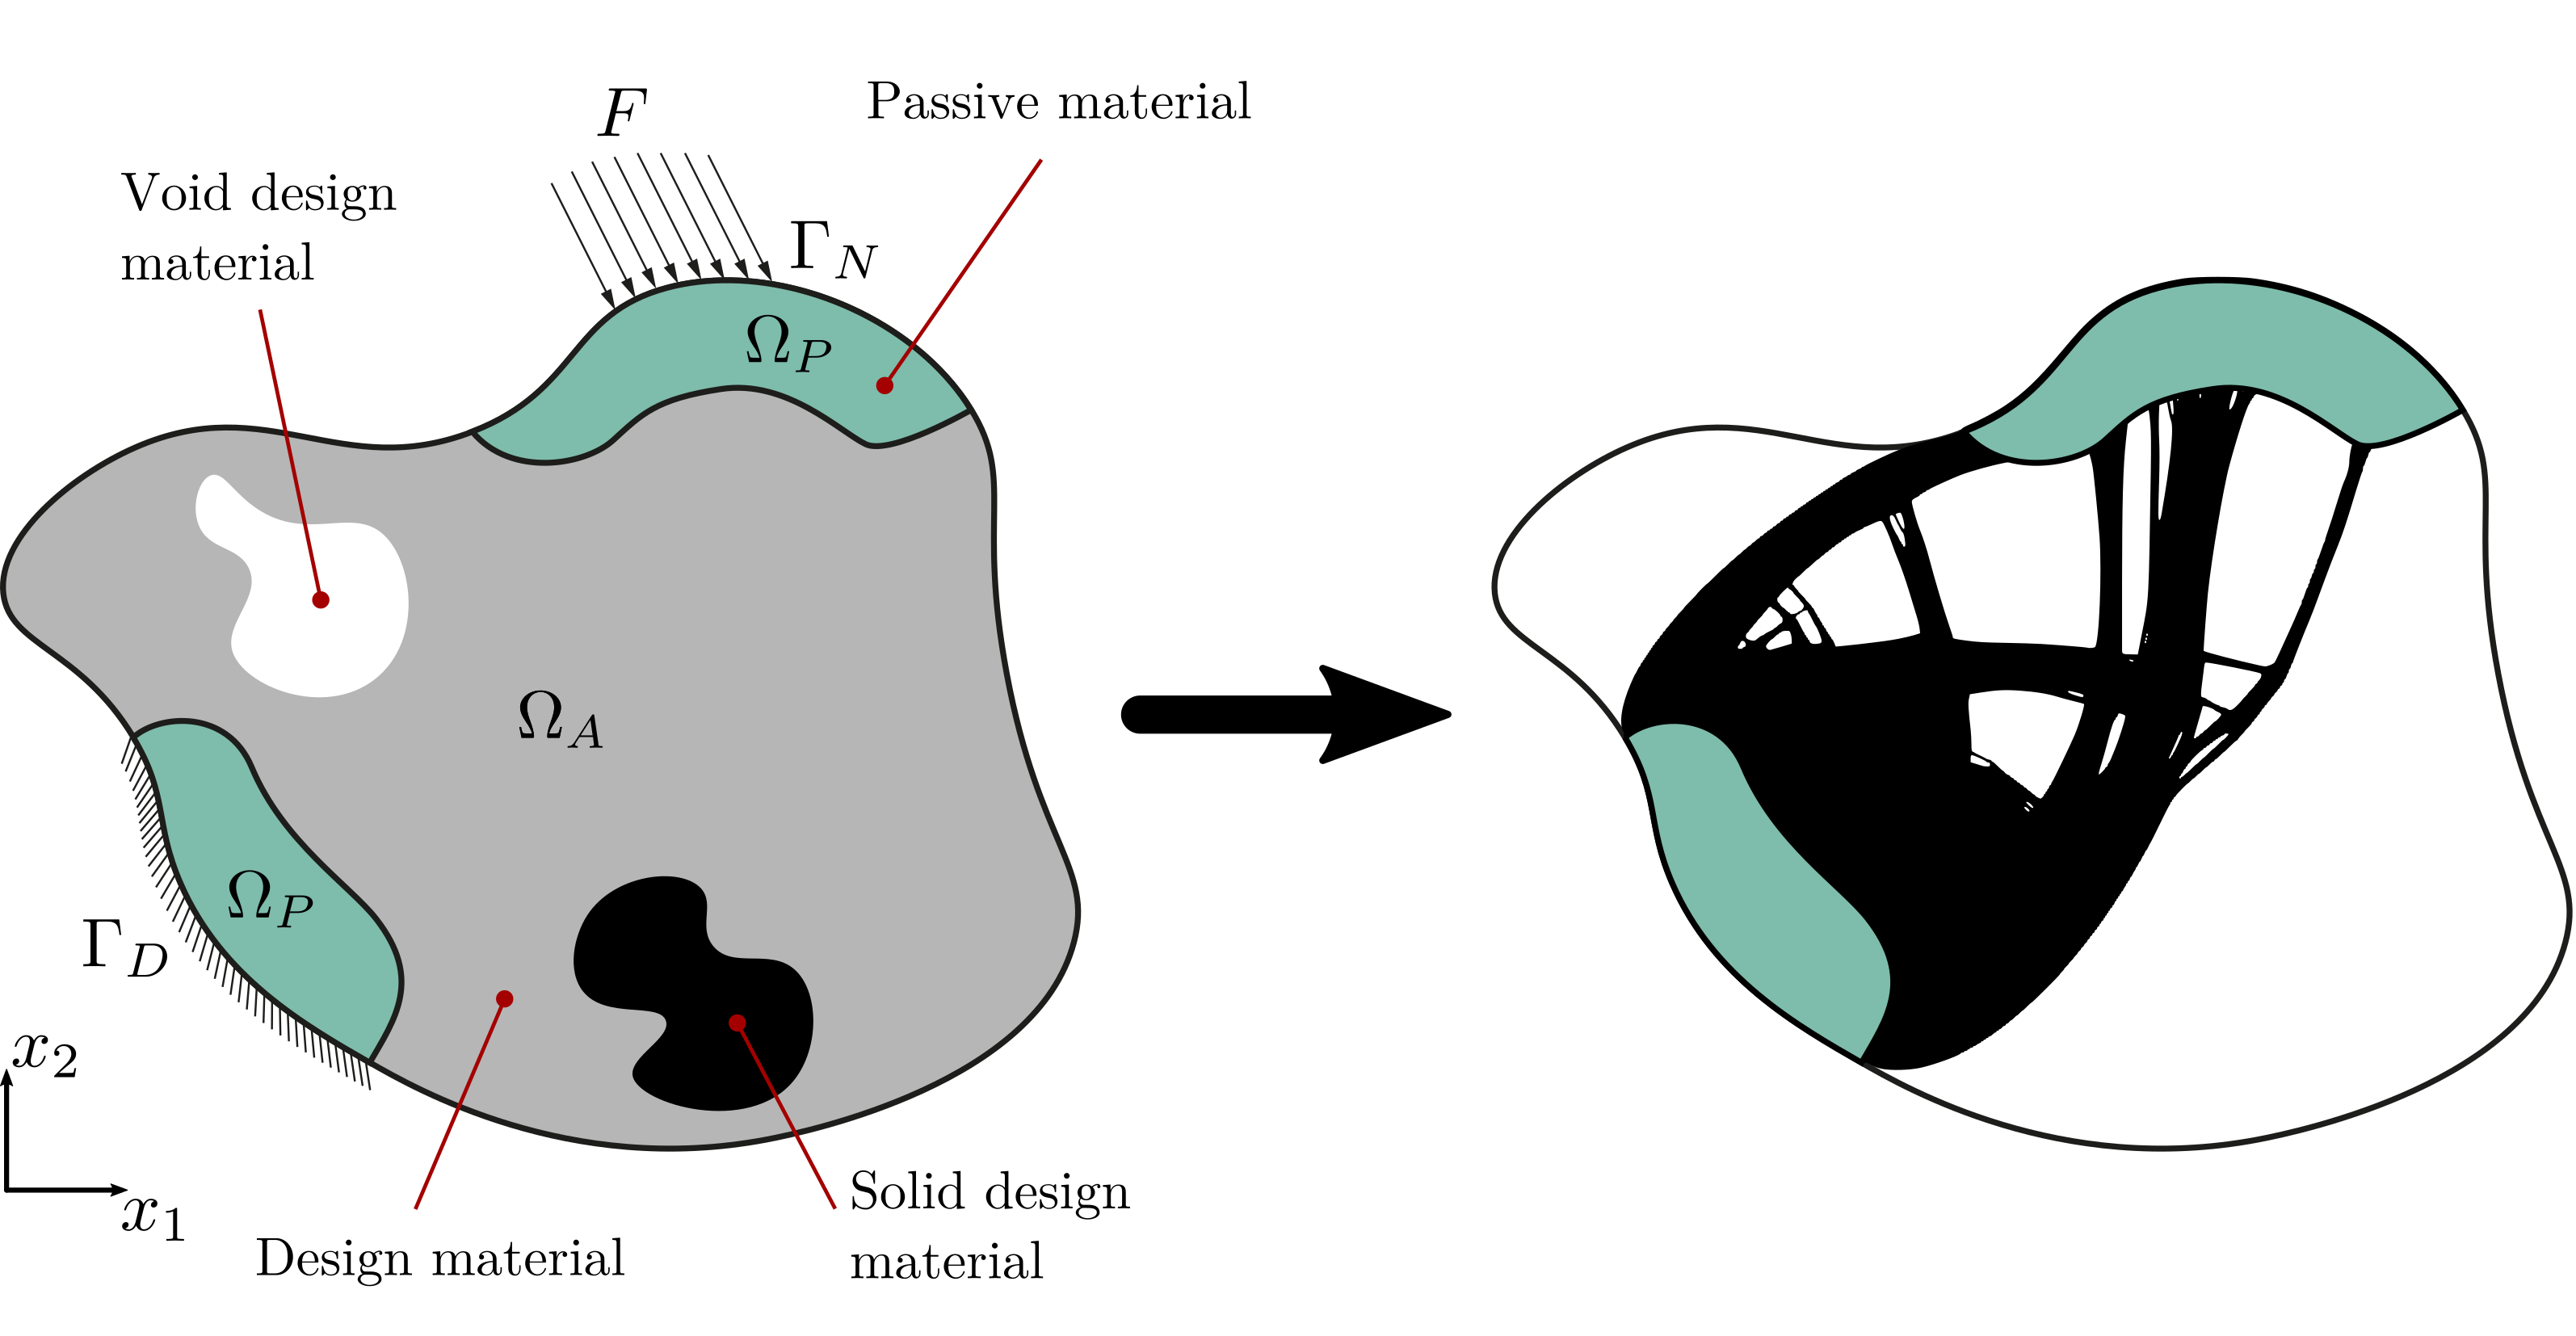
\includegraphics[width=1\imwidth]{figures/simpModel.png}}%
%    \caption{Bla bla bla...}
%    \label{fig:illustateTopOpt}
%\end{figure}


%\begin{equation}
%    (EIu'')'' = q
%\end{equation}


%\begin{figure}[tb]
%    \centering
%    \makebox[\textwidth][c]{\begin{tikzpicture}[remember picture]
    \begin{scope}[xshift=0mm]
        % angle (deg)
        \newcommand\ai{10}
        % line width
        \newcommand\wi{1pt}
        % cell size
        \newcommand\cellsize{3}
        % Rank-$N$ size
        \newcommand\di{0.75}

        % cell
        \draw[gray!10,   fill=gray!10, rotate around={\ai:(0,0)}] (0,0) rectangle (\cellsize,\cellsize) node (rect1) {};
        \draw[black!60, fill=black!60, rotate around={\ai:(0,0)}] (0,0) rectangle (\di,\cellsize);

        % orientation frame
        \draw[black, -stealth, line width=\wi, rotate around={\ai:({\di*cos(\ai) - \cellsize/2*sin(\ai)},{\di*sin(\ai) + \cellsize/2*cos(\ai)})}] ({\di*cos(\ai) - \cellsize/2*sin(\ai)},{\di*sin(\ai) + \cellsize/2*cos(\ai)}) -- ({\di*cos(\ai) - \cellsize/2*sin(\ai) + 0.75},{\di*sin(\ai) + \cellsize/2*cos(\ai)});
        \draw[black, -stealth, line width=\wi, rotate around={\ai:({\di*cos(\ai) - \cellsize/2*sin(\ai)},{\di*sin(\ai) + \cellsize/2*cos(\ai)})}] ({\di*cos(\ai) - \cellsize/2*sin(\ai)},{\di*sin(\ai) + \cellsize/2*cos(\ai)}) -- ({\di*cos(\ai) - \cellsize/2*sin(\ai)},{\di*sin(\ai) + \cellsize/2*cos(\ai) + 0.75});

        % local frame
        \draw[black, -stealth, dashed, line width=\wi] (0,0) -- ({\cellsize + 0.8},0);
        \draw[black, -stealth, dashed, line width=\wi] (0,0) -- (0,{\cellsize + 0.8});

        % ruler
        \draw[black, |-|, line width=\wi, rotate around={\ai:(0,0)}] (0,0) -- (\cellsize,0);
        \draw[black,  -|, line width=\wi, rotate around={\ai:(0,0)}] (0,0) -- (\di,0);

        % arc
        \draw[black, dotted, line width=\wi] (\cellsize,0) arc (0:\ai:\cellsize);

        % annotation
        \draw (\cellsize + 0.7, -0.3) node {$x_1 / \epsilon^3$};
        \draw (-0.5, \cellsize + 0.8) node {$x_2 / \epsilon^3$};
        \draw (\cellsize/2,-0.75) node {Rank-$1$};

        \draw[rotate around={{\ai/2}:(0,0)}] ({\cellsize+0.3},0) node {$\theta_1$};

        \draw[rotate around={{\ai}:(0,0)}] ({\di/2},0.4) node [rotate around={{\ai}:(0,0)}] {$\mu_1$};
        \draw[rotate around={{\ai}:(0,0)}] ({(\cellsize - \di)/2 + \di},0.4) node [rotate around={{\ai}:(0,0)}] {$1-\mu_1$};

        \draw[rotate around={{\ai}:(0,0)}] ({0+0.4},{\cellsize-0.4}) node [rotate around={{\ai}:(0,0)}] {$(+)$};
        \draw[rotate around={{\ai}:(0,0)}] ({\cellsize-0.4},{\cellsize-0.4}) node [rotate around={{\ai}:(0,0)}] {$(-)$};
        \coordinate (A) at (rect1.north);


        \draw[rotate around={\ai:({\di*cos(\ai) - \cellsize/2*sin(\ai)},{\di*sin(\ai) + \cellsize/2*cos(\ai)})}] ({\di*cos(\ai) - \cellsize/2*sin(\ai)+1} , {\di*sin(\ai) + \cellsize/2*cos(\ai) + 0.2}) node {$\mathbf{n}_1$};
        \draw[rotate around={\ai:({\di*cos(\ai) - \cellsize/2*sin(\ai)},{\di*sin(\ai) + \cellsize/2*cos(\ai)})}] ({\di*cos(\ai) - \cellsize/2*sin(\ai) + 0.3} , {\di*sin(\ai) + \cellsize/2*cos(\ai) + 1}) node {$\mathbf{m}_1$};



    \end{scope}
    \begin{scope}[xshift=45mm]
        % angle (deg)
        \newcommand\ai{15}
        % line width
        \newcommand\wi{1pt}
        % cell size
        \newcommand\cellsize{3}
        % Rank-$N$ size
        \newcommand\di{0.6}

        % cell
        \draw[gray!40,   fill=gray!40, rotate around={\ai:(0,0)}] (0,0) rectangle (\cellsize,\cellsize) node (rect2) {};
        \draw[black!60, fill=black!60, rotate around={\ai:(0,0)}] (0,0) rectangle (\di,\cellsize);

        % orientation frame
        \draw[black, -stealth, line width=\wi, rotate around={\ai:({\di*cos(\ai) - \cellsize/2*sin(\ai)},{\di*sin(\ai) + \cellsize/2*cos(\ai)})}] ({\di*cos(\ai) - \cellsize/2*sin(\ai)},{\di*sin(\ai) + \cellsize/2*cos(\ai)}) -- ({\di*cos(\ai) - \cellsize/2*sin(\ai) + 0.75},{\di*sin(\ai) + \cellsize/2*cos(\ai)});
        \draw[black, -stealth, line width=\wi, rotate around={\ai:({\di*cos(\ai) - \cellsize/2*sin(\ai)},{\di*sin(\ai) + \cellsize/2*cos(\ai)})}] ({\di*cos(\ai) - \cellsize/2*sin(\ai)},{\di*sin(\ai) + \cellsize/2*cos(\ai)}) -- ({\di*cos(\ai) - \cellsize/2*sin(\ai)},{\di*sin(\ai) + \cellsize/2*cos(\ai) + 0.75});

        % local frame
        \draw[black, -stealth, dashed, line width=\wi] (0,0) -- ({\cellsize + 0.8},0);
        \draw[black, -stealth, dashed, line width=\wi] (0,0) -- (0,{\cellsize + 0.8});

        % ruler
        \draw[black, |-|, line width=\wi, rotate around={\ai:(0,0)}] (0,0) -- (\cellsize,0);
        \draw[black,  -|, line width=\wi, rotate around={\ai:(0,0)}] (0,0) -- (\di,0);

        % arc
        \draw[black, dotted, line width=\wi] (\cellsize,0) arc (0:\ai:\cellsize);

        % annotation
        \draw (\cellsize + 0.7, -0.3) node {$x_1 / \epsilon^2$};
        \draw (-0.5, \cellsize + 0.8) node {$x_2 / \epsilon^2$};
        \draw (\cellsize/2,-0.75) node {Rank-$2$};

        \draw[rotate around={{\ai/2}:(0,0)}] ({\cellsize+0.3},0) node {$\theta_2 + \pi/4$};

        \draw[rotate around={{\ai}:(0,0)}] ({\di/2},0.4) node [rotate around={{\ai}:(0,0)}] {$\mu_2$};
        \draw[rotate around={{\ai}:(0,0)}] ({(\cellsize - \di)/2 + \di},0.4) node [rotate around={{\ai}:(0,0)}] {$1-\mu_2$};

        \draw[rotate around={{\ai}:(0,0)}] ({0+0.4},{\cellsize-0.4}) node [rotate around={{\ai}:(0,0)}] {$(+)$};
        \draw[rotate around={{\ai}:(0,0)}] ({\cellsize-0.9},{\cellsize-0.4}) node [rotate around={{\ai}:(0,0)}] (B) {$(\text{Rank-1})$};
        \coordinate (B2) at (rect2.north);


        \draw[rotate around={\ai:({\di*cos(\ai) - \cellsize/2*sin(\ai)},{\di*sin(\ai) + \cellsize/2*cos(\ai)})}] ({\di*cos(\ai) - \cellsize/2*sin(\ai)+1} , {\di*sin(\ai) + \cellsize/2*cos(\ai) + 0.2}) node {$\mathbf{n}_2$};
        \draw[rotate around={\ai:({\di*cos(\ai) - \cellsize/2*sin(\ai)},{\di*sin(\ai) + \cellsize/2*cos(\ai)})}] ({\di*cos(\ai) - \cellsize/2*sin(\ai) + 0.3} , {\di*sin(\ai) + \cellsize/2*cos(\ai) + 1}) node {$\mathbf{m}_2$};


    \end{scope}
    \begin{scope}[xshift=90mm]
        % angle (deg)
        \newcommand\ai{20}
        % line width
        \newcommand\wi{1pt}
        % cell size
        \newcommand\cellsize{3}
        % Rank-$N$ size
        \newcommand\di{1.0}

        % cell
        \draw[gray!60,   fill=gray!60, rotate around={\ai:(0,0)}] (0,0) rectangle (\cellsize,\cellsize);
        \draw[black!60, fill=black!60, rotate around={\ai:(0,0)}] (0,0) rectangle (\di,\cellsize);

        % orientation frame
        \draw[black, -stealth, line width=\wi, rotate around={\ai:({\di*cos(\ai) - \cellsize/2*sin(\ai)},{\di*sin(\ai) + \cellsize/2*cos(\ai)})}] ({\di*cos(\ai) - \cellsize/2*sin(\ai)},{\di*sin(\ai) + \cellsize/2*cos(\ai)}) -- ({\di*cos(\ai) - \cellsize/2*sin(\ai) + 0.75},{\di*sin(\ai) + \cellsize/2*cos(\ai)});
        \draw[black, -stealth, line width=\wi, rotate around={\ai:({\di*cos(\ai) - \cellsize/2*sin(\ai)},{\di*sin(\ai) + \cellsize/2*cos(\ai)})}] ({\di*cos(\ai) - \cellsize/2*sin(\ai)},{\di*sin(\ai) + \cellsize/2*cos(\ai)}) -- ({\di*cos(\ai) - \cellsize/2*sin(\ai)},{\di*sin(\ai) + \cellsize/2*cos(\ai) + 0.75});

        % local frame
        \draw[black, -stealth, dashed, line width=\wi] (0,0) -- ({\cellsize + 0.8},0);
        \draw[black, -stealth, dashed, line width=\wi] (0,0) -- (0,{\cellsize + 0.8});

        % ruler
        \draw[black, |-|, line width=\wi, rotate around={\ai:(0,0)}] (0,0) -- (\cellsize,0);
        \draw[black,  -|, line width=\wi, rotate around={\ai:(0,0)}] (0,0) -- (\di,0);

        % arc
        \draw[black, dotted, line width=\wi] (\cellsize,0) arc (0:\ai:\cellsize);

        % annotation
        \draw (\cellsize + 0.7, -0.3) node {$x_1 / \epsilon$};
        \draw (-0.5, \cellsize + 0.8) node {$x_2 / \epsilon$};
        \draw (\cellsize/2,-0.75) node {Rank-$3$};

        \draw[rotate around={{\ai/2}:(0,0)}] ({\cellsize+0.3},0) node {$\theta_3 - \pi/2$};

        \draw[rotate around={{\ai}:(0,0)}] ({\di/2},0.4) node [rotate around={{\ai}:(0,0)}] {$\mu_3$};
        \draw[rotate around={{\ai}:(0,0)}] ({(\cellsize - \di)/2 + \di},0.4) node [rotate around={{\ai}:(0,0)}] {$1-\mu_3$};

        \draw[rotate around={{\ai}:(0,0)}] ({0+0.4},{\cellsize-0.4}) node [rotate around={{\ai}:(0,0)}] {$(+)$};
        \draw[rotate around={{\ai}:(0,0)}] ({\cellsize-0.9},{\cellsize-0.4}) node [rotate around={{\ai}:(0,0)}] (C) {$(\text{Rank-2})$};


        \draw[rotate around={\ai:({\di*cos(\ai) - \cellsize/2*sin(\ai)},{\di*sin(\ai) + \cellsize/2*cos(\ai)})}] ({\di*cos(\ai) - \cellsize/2*sin(\ai)+1} , {\di*sin(\ai) + \cellsize/2*cos(\ai) + 0.2}) node {$\mathbf{n}_3$};
        \draw[rotate around={\ai:({\di*cos(\ai) - \cellsize/2*sin(\ai)},{\di*sin(\ai) + \cellsize/2*cos(\ai)})}] ({\di*cos(\ai) - \cellsize/2*sin(\ai) + 0.3} , {\di*sin(\ai) + \cellsize/2*cos(\ai) + 1}) node {$\mathbf{m}_3$};

    \end{scope}
    \path[-latex,black,thick] (A) edge [bend left=50] (B);
    \path[-latex,black,thick] (B2) edge [bend left=50] (C);
\end{tikzpicture}}%
%    \caption{Bla bla bla...}
%    \label{fig:Rank}
%\end{figure}

\section{Multiphysics effects in nano-optics}

RECHECK THAT EVERYTHING HERE IS CORRECT AND MAKES SENSE. 

Nature offers a wide range of examples of nano-optical systems that exhibit 
multi-physics effects, see Figure 1.
For example, the wings of the butterfly exhibit structural coloration due to the
 interaction of light 
with nanostructures in the wing scales. The color of the wings can change due to
 mechanical motion, where the angle of incidence of light changes.
The opal is another example of a natural nano-optical system, where the color of the opal
changes due to the periodic structure of the crystal. The color of the opal can change
due to the angle of incidence of light, or due to temperature changes in the evironment, 
which can result in evaporation, changing the spacing between the crystal planes.
Another example of a nano-optical system is the soap bubble, where the color of the bubble
changes due to the varying thickness of the bubble. The color of the bubble can change due to
mechanical stresses, evaporation due to temperature changes, or due to the chemical composition
of the bubble.
%butterfly example, chameleon, firefly bioluminesce with heat, opal iridescence (change with heat/water).
%Soap bubles, they will change color when through mechanical stresses, evaporation due to temperature changes, chemical composition, etc.

\begin{figure}[tb]
    \centering
    \makebox[\textwidth][c]{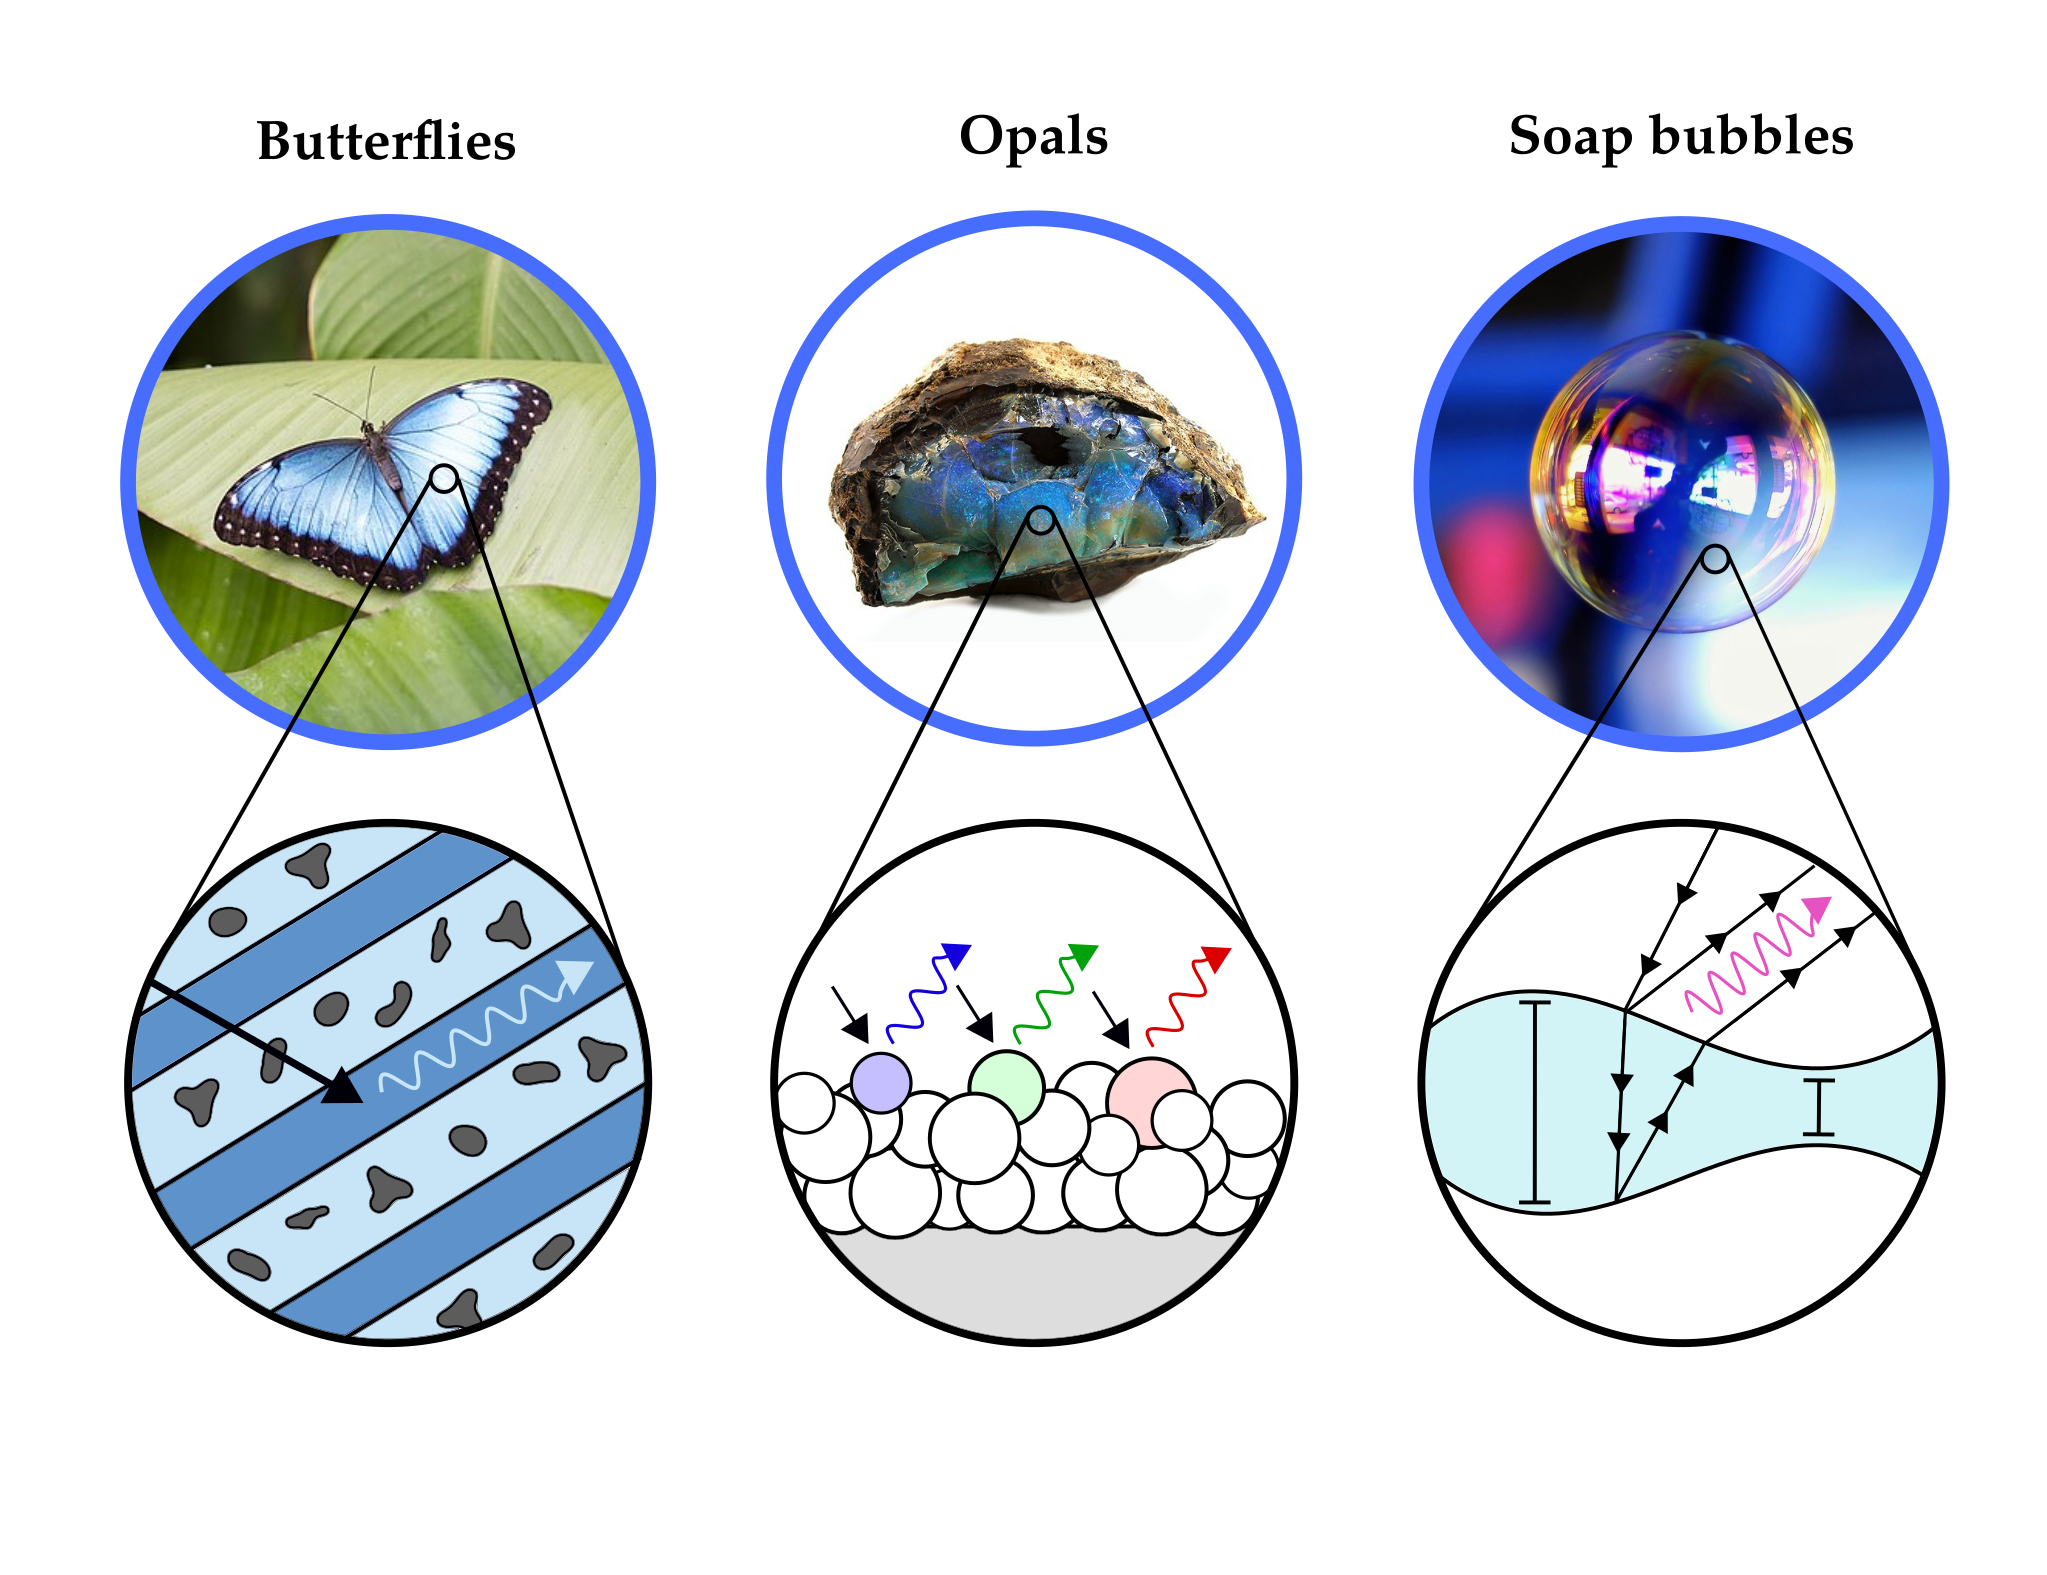
\includegraphics{figures/motivation_natural.png}}%%
    \caption{Examples of mascroscopic nano-optical systems that exhibit multi-physics effects. From left to right, nanostructures in wings of the butterfly, the colloidal crystal structure in the opal, and the thin-film effects in the varying thickness soap bubble.
    two colors in the soap bubble would work better visually! (Jens)}
    \label{fig:motivation_natural}
\end{figure}

% Wikimedia commons:
% 1. https://commons.wikimedia.org/wiki/File:Peleides_blue_morpho_(Morpho_peleides).jpg
% 2. https://commons.wikimedia.org/wiki/File:Opal-53714.jpg
% https://www.reddit.com/r/educationalgifs/comments/56sg9x/a_butterflys_wings_can_change_color_when_soaked/
%Sources:
%The GIF came from this video

%Ding, Y. Structural colors from Morpho peleides butterfly wing scales. J. Appl. Phys. 2009: 106, 074702

%Van Hooijdonk, E., et al. Detailed experimental analysis of the structural fluorescence in the butterfly Morpho sulkowskyi (Nymphalidae) J. Nanophoton. 2011: 5(1), 053525


The field of nano-optics ...

\section{Topology optimization in nano-optics}

As seen by the examples in Figure 1, nano-optical systems exhibit multi-physics effects,
where ingenously engineered geometry and material properties play a crucial role in the
optical response of the system. Inspired by these natural structures a goal of nano-optics
design is to optimize the geometry and material properties of the system to achieve a desired
optical response. Topology optimization offers a systematic approach to optimize the geometry
and material properties of a system to obtain a desired optical performance under a set of constraints.

Topology optimization is a systematic design method that can optimize designs based on a target FOM and a set of constraints. 
Say that it was introduced in the field of mechanics (CITE BENDSOE), but then it was extended to 
nano-optic and nanphotonic systems (CITE JENSEN, SIGMUND).

In Figure XX we we show an example of a topology optimziation problem in nano-optics. The 
main idea is two optimize the distribution of material in the design domain for two different materials, 
where the material distribution is optimized to maximize a FOM. ADD SOMETHING ABOUT THE SOURCE.


\begin{figure}[tb]
    \centering
    \makebox[\textwidth][c]{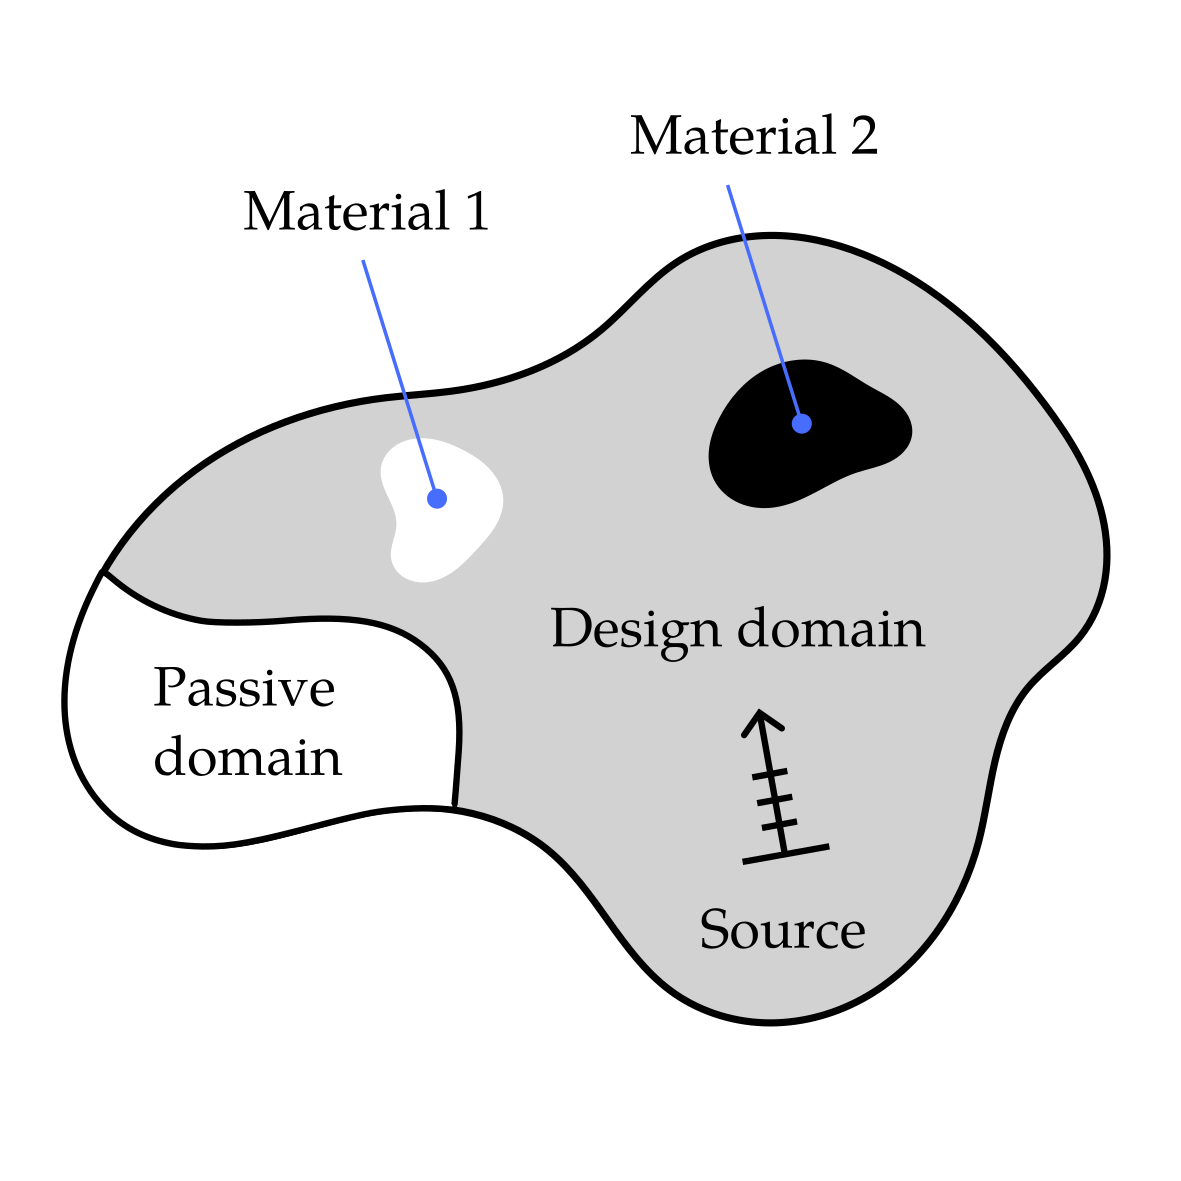
\includegraphics{figures/top_opt.png}}%%
    \caption{Topology optimization of a nano-optic system, excited by a source. The simulation domain is composed by a passive domain (blue) where the material is fixed, and a design domain (grey), where the material distribution is optimized for two different materials.}
    \label{fig:top_opt}
\end{figure}

\section{Structure of the Thesis}

This thesis covers multi-physics topology optimization problems in nano-optic systems. It provides an overview
of different type of multi-physics problems.

\textbf{Chapter 1} presents ...

\textbf{Chapter 2} presents ...

This thesis consists of a collection of papers, including unpublished work on
systems of coupled dipole emitter problems. The published content is included in the attached
papers.


\newrefcontext[labelprefix=]
\printbibliography[notkeyword=myPub,notkeyword=myMan]


\appendix
\chapter{Appendix}
\section{Sensitivity analysis for weakly coupled multiphysics problems}\label{app:appendix1}
In this appendix, we derive the adjoint sensitivity expressions for a general weakly coupled multiphysics
 problem with $N$ physics. The system is written as $\mathbf{K}\mathbf{u} = \mathbf{f}$, where $\mathbf{K}$ is 
 the stiffness matrix of the coupled system, $\mathbf{u}$ is the solution vector, and $\mathbf{f}$ is the source or forcing term vector. For 
 simplicity, we assume real-valued problems, but this method can be extended to complex-valued cases, as shown
  in~\cite{ownpub0} for a simple two-physics ($N=2$) example. As described in~\secref{sec:coupled}, 
  for $N$ physics with \textbf{weak nonlinear coupling} (\eqref{eq:multiphysics_weak_nonlinear}), the full 
  system is upper or lower triangular, as in
\begin{equation} \label{eq:app_multiphysics_weak}
    \begin{bmatrix}
        \mathbf{K}_1(\mathbf{u}_2, \cdots \mathbf{u}_N)    & \mathbf{C}_{12} (\mathbf{u}_2, \cdots \mathbf{u}_N)& \cdots & \mathbf{C}_{1N}(\mathbf{u}_2, \cdots \mathbf{u}_N) \\
        0 & \mathbf{K}_2 (\mathbf{u}_3, \cdots \mathbf{u}_N)   & \cdots & \mathbf{C}_{2N} (\mathbf{u}_3, \cdots \mathbf{u}_N)\\
        \vdots          & \vdots          & \ddots & \vdots          \\
        0& 0 & \cdots & \mathbf{K}_N
    \end{bmatrix}
    \begin{bmatrix}
        \mathbf{u}_1 \\
        \mathbf{u}_2 \\
        \vdots       \\
        \mathbf{u}_N
    \end{bmatrix}
    =
    \begin{bmatrix}
        \mathbf{f}_1\\
        \mathbf{f}_2\\
        \vdots       \\
        \mathbf{f}_N
    \end{bmatrix}\,,
\end{equation}
where we have chosen the upper diagonal version of the weakly coupled problem and the system of equations has been rewriten in terms of the stiffness ($\mathbf{K}_i$) and 
coupling matrices ($\mathbf{C}_{ij}$) so that the right-hand-side $\mathbf{f}=[\mathbf{f}_1, \cdots, \mathbf{f}_N]^\top$ does not depend
on the solution vector $\mathbf{u}=[\mathbf{u}_1, \cdots, \mathbf{u}_N]^\top$. This notation is equivalent to having $N$ equations of the form
\begin{align}
\left\{
    \begin{aligned}
        \quad \mathbf{K}_1(\mathbf{u}_2, \ldots, \mathbf{u}_N)\, \mathbf{u}_1  + \sum_{j=2}^N \mathbf{C}_{1j} (\mathbf{u}_2, \cdots \mathbf{u}_N)\, \mathbf{u}_j &= \mathbf{f}_1\,, \\
        \quad\mathbf{K}_2(\mathbf{u}_3, \ldots, \mathbf{u}_N)\, \mathbf{u}_2 + \sum_{j=3}^N \mathbf{C}_{2j} (\mathbf{u}_3, \cdots \mathbf{u}_N)\, \mathbf{u}_j &= \mathbf{f}_2\,, \\
        \quad\ldots \\
        \quad\mathbf{K}_{N-1} (\mathbf{u}_N) \, \mathbf{u}_{N-1} + \mathbf{C}_{N-1\, N}(\mathbf{u}_N)\, \mathbf{u}_N &= \mathbf{f}_{N-1} \,, \\
        \quad\mathbf{K}_N \, \mathbf{u}_N &= \mathbf{f}_N\,.
    \end{aligned}
\right.
\end{align}
In this case, we can solve the system of equations sequentially in a \textbf{seggregated} fashion,
 where problem $i=N$ is solved first, and the solution is used to solve the next problem ($i=N-1$), and so on, until the first problem ($i=1$) is solved
 (as in the sequence: $\mathbf{u}_N \to \mathbf{u}_{N-1} \to \cdots \to \mathbf{u}_1$).\\

To calculate the sensitivites using the adjoint method we start by rewriting the FOM ($\Psi$) by adding the residual
of the state equations, multiplied by a set of Lagrange multipliers ($\Lambda_i$)
\begin{equation}\label{eq:adj_init}
    \Psi^\prime =\Psi + \sum^N_{i=1} \Lambda_{i}^{\top}\left(\mathbf{K}_i \mathbf{u}_i -\mathbf{f}_i + \sum^N_{j=i+1} \mathbf{C}_{ij} \mathbf{u}_j \right)\,.
\end{equation}
Now we calculate the sensitivities by taking the derivative of the FOM with respect to the physical field ($\hat{\rho}$)
\begin{align}\label{eq:sens_init}
    \frac{\d \Psi^\prime}{\d \hat{\rho}} 
    = \frac{\partial \Psi}{\partial \hat{\rho}} 
    &+ \sum_{i=1}^N \mathcal{D}^{(i)}[\Psi]
    + \sum_{i=1}^N \Lambda_i^\top \Bigg\{\Bigg(
        \frac{\partial \mathbf{K}_i}{\partial \hat{\rho}} 
        + \mathcal{D}^{(i+1)}[\mathbf{K}_i]\Bigg) \mathbf{u}_i 
        + \mathbf{K}_i \mathcal{D}^{(i)}[\mathbf{u}_i] \nonumber \\
        - \frac{\partial \mathbf{f}_i}{\partial \hat{\rho}} 
        &+ \sum_{j=i+1}^{N} \Bigg[ \Bigg(
            \frac{\partial \mathbf{C}_{ij}}{\partial \hat{\rho}} + 
            \mathcal{D}^{(i+1)}[\mathbf{C}_{ij}] \Bigg)\, \mathbf{u}_j 
            + \mathbf{C}_{ij} \mathcal{D}^{(j)}[\mathbf{u}_j] 
        \Bigg]
    \Bigg\}. 
\end{align}
where we have defined $\mathcal{D}^{(i)}[a]$ as the cascaded differential operator acting on $a$ to compactly write the derivative
\begin{align}
    \hspace*{-0.775cm}\mathcal{D}^{(i)}[a] &= \sum^N_{i} \frac{\partial a}{\partial \mathbf{u}_i} \Bigg[ \frac{\partial \mathbf{u}_i}{\partial \hat{\rho}} + 
    \sum_{j=i+1}^{N} \frac{\partial \mathbf{u}_i}{\partial \mathbf{u}_j} \Bigg( \frac{\partial \mathbf{u}_j}{\partial \hat{\rho}} + 
    \sum_{k=j+1}^{N} \frac{\partial \mathbf{u}_j}{\partial \mathbf{u}_k} \Bigg( \frac{\partial \mathbf{u}_k}{\partial \hat{\rho}} + \cdots \Bigg) \Bigg) \Bigg] \,\,\,\, \forall i \in [1, N] \,.
\end{align}
The chain-rule-based derivative expression in \eqref{eq:sens_init} takes into account all the dependencies of the solutions in the weakly coupled problem (\eqref{eq:app_multiphysics_weak}).

Taking \autoref{eq:sens_init} and grouping the terms it is possible to rewrite the sensitivities as
\begin{align}
    \frac{\d \Psi^\prime}{\d \hat{\rho}}  &= \frac{\partial \Psi}{\partial \hat{\rho}} + \sum^N_{i=1} \Lambda_{i}^{\top} \left( \frac{\partial \mathbf{K}_i}{\partial \hat{\rho}} \mathbf{u}_i - \frac{\partial \mathbf{f}_i}{\partial \hat{\rho}} + \sum_{j=i+1}^{N} \frac{\partial \mathbf{C}_{ij}}{\partial \hat{\rho} } \mathbf{u}_j \right) + \\ &+ \frac{\partial \mathbf{u}_1}{\partial \hat{\rho}} \big( \mathcal{A}_1 \big) + \frac{\partial \mathbf{u}_2}{\partial \hat{\rho}} \left( \mathcal{A}_1 \frac{\partial \mathbf{u}_1}{\partial \mathbf{u}_2} + \mathcal{A}_2 \right) + \\
    &+ \frac{\partial \mathbf{u}_3}{\partial \hat{\rho}} \left[ \mathcal{A}_1 \left( \frac{\partial \mathbf{u}_1}{\partial \mathbf{u}_3} + \frac{\partial \mathbf{u}_2}{\partial \mathbf{u}_3}\frac{\partial \mathbf{u}_1}{\partial \mathbf{u}_2}\right) + \frac{\partial \mathbf{u}_2}{\partial \mathbf{u}_3} \mathcal{A}_2 + \mathcal{A}_3 \right] + \cdots
\end{align}
where $\mathcal{A}_i (\Lambda_i)$ are the adjoint equation terms
\begin{equation}
    \mathcal{A}_i = \frac{\partial \Psi}{\partial \mathbf{u}_i} + \Lambda_{i}^\top \mathbf{K}_i + \sum_{j=1}^{i-1} \Lambda_j^\top\left(
     \frac{\partial \mathbf{K}_j}{\partial \mathbf{u}_i}\mathbf{u}_j + \mathbf{C}_{ji} + \sum^N_{k=j+1} \frac{\partial \mathbf{C}_{jk}}{\partial \mathbf{u}_i} \mathbf{u}_k  \right) \quad \quad \forall i \in [1, N] \,,
\end{equation}
which can be set to zero ($\mathcal{A}_i=0$) by solving the adjoint problems. 
To solve the adjoint equations one needs to find the Lagrange multipliers $\Lambda_i$ as the solution to the adjoint equations
\begin{equation}\label{eq:app_adj_eqs}
     \mathbf{K}^\top_i \Lambda_i = -\left(\frac{\partial \Psi}{\partial \mathbf{u}_i}\right)^\top - \sum_{j=1}^{i-1} \left[ 
     \mathbf{u}^\top_j \left(\frac{\partial \mathbf{K}_j}{\partial \mathbf{u}_i}\right)^\top + \mathbf{C}^\top_{ji} + \sum^N_{k=j+1} \mathbf{u}^\top_k \left(\frac{\partial \mathbf{C}_{jk}}{\partial \mathbf{u}_i}\right)^\top \right]\Lambda_j  \quad \forall i \in [1, N] \,,
\end{equation}
thus yielding the final expression for the sensitivities
\begin{equation}
    \frac{\d \Psi^\prime}{\d \hat{\rho}}  = \frac{\partial \Psi}{\partial \hat{\rho}} + \sum^N_{i=1} \Lambda_{i}^{\top} \left( \frac{\partial \mathbf{K}_i}{\partial \hat{\rho}} \mathbf{u}_i - \frac{\partial \mathbf{f}_i}{\partial \hat{\rho}} + \sum^N_{j=i+1} \frac{\partial \mathbf{C}_{ij}}{\partial \hat{\rho}} \mathbf{u}_j \right)\,.
\end{equation}
This means that the adjoint equations in \eqref{eq:app_adj_eqs} are solved in reverse order with respect to the forward solution (\eqref{eq:app_multiphysics_weak}). In other words, one needs to solve the first adjoint equation ($i=1$) 
and feed the solution the next adjoint equation ($i=2$), and so on, to solve the last adjoint problem $i=N$  (as in the sequence: $\Lambda_1 \to \Lambda_{2} \to \cdots \to \Lambda_N$).

% In the sequential case, the solutions of the different physics couple one-to-one in a seggregated fashion (
% $\mathbf{u}_1 \to \mathbf{u}_2 \to \cdots \to \mathbf{u}_N$)
% and there is no other coupling mechanism between the physics. In this case the system of equations can be written as in Eq.~\eqref{eq:multiphysics_weak}.



% In this case, taking the derivative of the FOM with respect to the design variable $\xi$:
% \begin{equation}\label{eq:adj_seq}
%     \frac{\d \tilde{\Phi}}{\d \xi} = \frac{\partial \Phi}{\partial \xi} + \mathcal{D}^{(1)}_\circ \left[\Phi\right] + 
%     \sum^N_i \lambda_{i}^{\top} \left[ \left(\frac{\partial \mathbf{S}_i}{\partial \xi} +  \mathcal{D}^{(i)}_\circ \left[\mathbf{S}_i\right]\right) \mathbf{u}_i
%     + \mathbf{S}_i \mathcal{D}^{(i)}_\circ \left[\mathbf{u}_i\right] - \frac{\partial \mathbf{f}_i}{\partial \xi }\right]
% \end{equation}
% where we have defined $\mathcal{D}^{(i)}_\circ[a]$ as the sequential or composition ($\circ$) differential operator acting on $a$ to compactly write the derivative:
% \begin{align}
%     \mathcal{D}^{(i)}_\circ[a] &= \frac{\partial a}{\partial \mathbf{u}_i} \sum_{j=i}^{N} \frac{\partial \mathbf{u}_j}{\partial \xi} 
%         \prod_{k \leq j}^{j} \frac{\partial \mathbf{u}_k}{\partial \mathbf{u}_{k+1}}\,, \\
%         &= \frac{\partial a}{\partial \mathbf{u}_i} \left( \frac{\partial \mathbf{u}_i}{\partial \xi} + 
%             \frac{\partial \mathbf{u}_i}{\partial \mathbf{u}_{i+1}} \left( \frac{\partial \mathbf{u}_{i+1}}{\partial \xi} + 
%                 \frac{\partial \mathbf{u}_{i+1}}{\partial \mathbf{u}_{i+2}} \left( \frac{\partial \mathbf{u}_{i+2}}{\partial \xi} + 
%                     \cdots
%                 \right)
%             \right)
%         \right) \,.
%     \end{align}
% Using Eq.~\eqref{eq:adj_seq} and grouping the terms:
% \begin{equation}
%     \frac{\d \tilde{\Phi}}{\d \xi} =  \frac{\partial \Phi}{\partial \xi} + \sum_i \lambda_{i}^{\top} \left( \frac{\partial \mathbf{S}_i}{\partial \xi} \mathbf{u}_i - \frac{\partial \mathbf{f}_i}{\partial \xi} \right)
%     + \sum^{N-1}_{i=1}  \frac{\partial \mathbf{u}_{i}}{\partial \xi} \left( \lambda_{i}^{\top} \frac{\partial \mathbf{S}_i}{\partial \mathbf{u}_{i+1}}\mathbf{u}_{i}
%     +  \lambda_{i+1}^{\top} \mathbf{S}_{i+1}\right)\,.
% \end{equation}
% We can by choose the Lagrange multipliers to the last summation term is zero, by solving $N$ adjoint equations:
% \begin{align}
%     \mathbf{S}^\top_{1}\lambda_{1} &= - \frac{\partial \Phi}{\partial \mathbf{u}_{1}} \label{eq:seq_adj_1}\,\\
%     \mathbf{S}^\top_{i+1}\lambda_{i+1} &= - \mathbf{u}^\top_i \left(\frac{\partial \mathbf{S}_i}{\partial \mathbf{u}_{i+1}}\right)^\top \lambda_i \quad \forall i \in [1, N-1] \label{eq:seq_adj_N-1}\,,
% \end{align}
% where the adjoint equations imply a relationship where the coupling happens backwards. In other words, one needs to solve the first adjoint equation (Eq.~\eqref{eq:seq_adj_1}), 
% and feed the solution the next adjoint equation ($i=2$, Eq.~\eqref{eq:seq_adj_N-1}) (and so on); where the coupling is inverted with respect to the physics. Solving these adjoint equations we can calculate the lagrang
% multipliers which give the final sensitivities:
% \begin{equation}
%     \frac{\d \tilde{\Phi}}{\d \xi} = \frac{\partial \Phi}{\partial \xi} + \sum_i \lambda_{i}^{\top} \left( \frac{\partial \mathbf{S}_i}{\partial \xi} \mathbf{u}_i - \frac{\partial \mathbf{f}_i}{\partial \xi} \right)\,.
% \end{equation}

% \subsection{Parallel coupling}

% Let's now consider the case of parallel coupling, where the solution of $N-1$ physics are coupled solve the last ($i=1$) physics ($[\mathbf{u}_2, \mathbf{u}_3, \cdots, \mathbf{u}_{N-1}] \to \mathbf{u}_1$). By reusing Eq.~\eqref{eq:adj_seq},
% we can now take the derivative with respect to the design variables:
% \begin{align}\label{eq:adj_parallel}
%     \frac{\d \tilde{\Phi}}{\d \xi} &= \frac{\partial \Phi}{\partial \xi} + \mathcal{D}^{(1)}_\parallel \left[\Phi\right]  
%     +  \lambda_{1}^{\top} \left[\left( \frac{\partial \mathbf{S}_1}{\partial \xi} +  \mathcal{D}^{(1)}_\parallel \left[\mathbf{S}_1\right] \right) \mathbf{u}_1
%     + \mathbf{S}_1  \mathcal{D}^{(1)}_\parallel \left[\mathbf{u}_1\right] \right] + \\
%     &+ \sum_{i=2}^{N} \lambda_{i}^{\top} \left( \frac{\partial \mathbf{S}_i}{\partial \xi}\mathbf{u}_i + \mathbf{S}_i \frac{\partial \mathbf{u}_i}{\partial \xi} - \frac{\partial \mathbf{f}_i}{\partial \xi}\right)
% \end{align}
% where we have defined $\mathcal{D}^{(i)}_\parallel[a]$ as the parallel ($\parallel$) differential operator acting on $a$ to compactly write the derivative:
% \begin{equation}
%     D^{(i)}_\parallel[a] = \frac{\partial a}{\partial \mathbf{u}_i} \sum_{j=1}^{N} \frac{\partial \mathbf{u}_j}{\partial \mathbf{u}_i} 
%     \frac{\partial \mathbf{u}_j}{\partial \xi}\,.
% \end{equation}
% Using Eq.~\eqref{eq:adj_parallel} and grouping the terms:
% \begin{equation}
%     \frac{\d \tilde{\Phi}}{\d \xi} = \frac{\partial \Phi}{\partial \xi} + \sum_i \lambda_{i}^{\top} \left( \frac{\partial \mathbf{S}_i}{\partial \xi} \mathbf{u}_i - \frac{\partial \mathbf{f}_i}{\partial \xi} \right)
%     + \frac{\partial \mathbf{u}_1}{\partial \xi} \left( \lambda_{1}^{\top}  \mathbf{S}_1 + \frac{\partial \Phi}{\partial \mathbf{u}_1} \right) + 
%     \sum^{N}_{i=2} \left( \lambda_{i}^{\top} \mathbf{S}_i + \lambda_{1}^{\top}  \frac{\partial \mathbf{S}_i}{\partial \mathbf{u}_1} \mathbf{u}_i\right)\,.
% \end{equation}
% We can by choose the Lagrange multipliers so that the last two terms are zero, by solving $N$ adjoint equations:
% \begin{align}
%     \mathbf{S}^\top_{1}\lambda_{1} &= - \frac{\partial \Phi}{\partial \mathbf{u}_{1}} \label{eq:par_adj_1}\,\\
%     \mathbf{S}^\top_{i}\lambda_{i} &= - \mathbf{u}^\top_1 \left(\frac{\partial \mathbf{S}_1}{\partial \mathbf{u}_i}\right)^\top \lambda_1 \quad \forall i \in [2, N] \label{eq:par_adj_N-1}\,,
% \end{align}
% The Lagrange multipliers are a solution to this equation and can be used to simplify the sensitivity expression:
% \begin{equation}
%     \frac{\d \tilde{\Phi}}{\d \xi} = \frac{\partial \Phi}{\partial \xi} + \sum_i \lambda_{i}^{\top} \left( \frac{\partial \mathbf{S}_i}{\partial \xi} \mathbf{u}_i - \frac{\partial \mathbf{f}_i}{\partial \xi} \right)\,.
% \end{equation}
% which is the same result as in the case of sequential coupling, with different Lagrange multipliers.

% \subsection{Generalizing to simultaenous sequential and parallel coupling}
% Based on the result from the previous sections, in the general coupling case, where there might be parallel and sequential couplings simultaneously, the sensitivities can be calculated as:
% \begin{equation}
%     \frac{\d \tilde{\Phi}}{\d \xi} = \frac{\partial \Phi}{\partial \xi} + \sum_i \lambda_{i}^{\top} \left( \frac{\partial \mathbf{S}_i}{\partial \xi} \mathbf{u}_i - \frac{\partial \mathbf{f}_i}{\partial \xi} \right)\,.
% \end{equation}
% The only difference is solution to the adjoint equations, which depends on the coupling. In the general case, where all couplings feed to a 
% final physics ($i=1$) but may be coupled in any combinations between each other, it can be shown that the adjoint equations are:
% \begin{align}
%     \mathbf{S}^\top_{1}\lambda_{1} &= - \frac{\partial \Phi}{\partial \mathbf{u}_{1}}\,\\
%     \mathbf{S}^\top_{i}\lambda_{i} &= - \sum^{C_i}_j \mathbf{u}^\top_j \left(\frac{\partial \mathbf{S}_j}{\partial \mathbf{u}_{i}}\right)^\top \lambda_j \quad \forall i \in [1, N-1]\, , \quad \forall j \in [1, C_i] \,.
% \end{align}
% where $C_i<N$ is the number of physics that are coupled to the $i$th physics, and where we have used that the problems are linear. 




\pagestyle{plain}

\FloatBarrier
\chapter*{Publications}
\addcontentsline{toc}{chapter}{Publications}%
\cleardoublepage
\vspace*{0.4\textheight}
\begin{center}
  \begin{minipage}{0.9\linewidth}
    \section*{Publication \cite{ownpub0}}
    \addcontentsline{toc}{section}{Publication \cite{ownpub0}}%

    Reprinted with permission from:\\ 

    \textbf{Beñat Martinez de Aguirre Jokisch}, Rasmus Ellebæk Christiansen, and Ole Sigmund. "Topology optimization framework for designing efficient thermo-optical phase shifters". \textit{J. Opt. Soc. Am. B} 41, A18-A31 (2024) [\textit{Published}]. \\
  
    © Optical Society of America.

  \end{minipage}
\end{center}
\newpage
\includepdf[pages=-,width=1.005\paperwidth, templatesize={\paperwidth}{\paperheight}, offset=1mm -0.7mm]{ownPub/ownpub0.pdf}
\cleardoublepage
\vspace*{0.4\textheight}
\begin{center}
  \begin{minipage}{0.9\linewidth}
    \section*{Publication \cite{ownpub1}}
    \addcontentsline{toc}{section}{Publication \cite{ownpub1}}%

    Reprinted with permission from:\\ 

    \textbf{Beñat Martinez de Aguirre Jokisch}, Benjamin Falkenberg Gøtzsche, Philip Trøst Kristensen, Martijn Wubs, Ole Sigmund, and Rasmus Ellebæk Christiansen. "Omnidirectional Gradient Force Optical Trapping in Dielectric Nanocavities by Inverse Design". \textit{ACS Photonics} 11 (12), 5118-5127 (2024) [\textit{Published}]. \\

    © 2024 American Chemical Society.\\

    Link to the published work (ACS Articles on Request):\\
     \url{https://pubs.acs.org/articlesonrequest/AOR-AMQAZZRW4FK6BSQGAT8X}
  \end{minipage}
\end{center}
\newpage
\includepdf[pages=-,width=1.005\paperwidth, templatesize={\paperwidth}{\paperheight}, offset=1mm -0.7mm]{ownPub/ownpub1.pdf}
\cleardoublepage
\vspace*{0.4\textheight}
\begin{center}
  \begin{minipage}{0.9\linewidth}
    \section*{Publication \cite{ownpub3}}
    \addcontentsline{toc}{section}{Publication \cite{ownpub3}}%

    © 2024 IEEE. Reprinted with permission from: \\


    \textbf{Beñat Martinez de Aguirre Jokisch}, Ole Sigmund, and Rasmus Ellebæk Christiansen. "Inverse design of dielectric nanostructures for optical trapping". \textit{Proc. SPIE 13112, Optical Trapping and Optical Micromanipulation XXI, 1311204} (2024) [\textit{Published}].
  \end{minipage}
\end{center}
\newpage
\includepdf[pages=-,width=1.005\paperwidth, templatesize={\paperwidth}{\paperheight}, offset=1mm -0.7mm]{ownPub/ownpub3.pdf}
\cleardoublepage
\vspace*{0.4\textheight}
\begin{center}
  \begin{minipage}{0.9\linewidth}
    \section*{Publication \cite{ownpub2}}
    \addcontentsline{toc}{section}{Publication \cite{ownpub2}}%
    Reprinted with permission from:\\ 

    \textbf{Beñat Martinez de Aguirre Jokisch}, Rasmus Ellebæk Christiansen, and Ole Sigmund. "Engineering optical forces through Maxwell stress tensor inverse design".  \textit{J. Opt. Soc. Am. B} 42, 731-741 (2025) [\textit{Published}].\\

    © Optical Society of America.

  \end{minipage}
\end{center}
\newpage
\includepdf[pages=-,width=1.005\paperwidth, templatesize={\paperwidth}{\paperheight}, offset=1mm -0.7mm]{ownPub/ownpub2.pdf}
\cleardoublepage
\vspace*{0.4\textheight}
\begin{center}
  \begin{minipage}{0.9\linewidth}
    \section*{Publication \cite{ownpub4}}
    \addcontentsline{toc}{section}{Publication \cite{ownpub4}}%
    \textbf{Beñat Martinez de Aguirre Jokisch}, Alexander Cerjan, Rasmus Ellebæk Christiansen, Jesper Mørk, Ole Sigmund, Steven G. Johnson. "Efficient first-principles inverse design of nanolasers". \textit{Laser \& Photonics Reviews} (2025) [\textit{Under Review}] .
  \end{minipage}
\end{center}
\newpage
\includepdf[pages=-,width=1.005\paperwidth, templatesize={\paperwidth}{\paperheight}, offset=1mm -0.7mm]{ownPub/ownpub4.pdf}
\cleardoublepage
\vspace*{0.4\textheight}
\begin{center}
  \begin{minipage}{0.9\linewidth}
    \section*{Publication \cite{ownpub5}}
    \addcontentsline{toc}{section}{Publication \cite{ownpub5}}%
    \textbf{Beñat Martinez de Aguirre Jokisch}, Rasmus Ellebæk Christiansen, Ole Sigmund. "Topology optimization in strongly coupled optomechanical systems". (2025) [\textit{In preparation}] .
  \end{minipage}
\end{center}
\newpage
\includepdf[pages=-,width=1.005\paperwidth, templatesize={\paperwidth}{\paperheight}, offset=1mm -0.7mm]{ownPub/ownpub5.pdf}

%\vspace*{0.4\textheight}
%\begin{center}
%  \begin{minipage}{0.9\linewidth}
%    \section*{Manuscript \cite{ownpub1}}
%    \addcontentsline{toc}{section}{Manuscript \cite{ownpub1}}%
%    Bla bla bla...
%  \end{minipage}
%\end{center}
%\newpage
%\includepdf[pages=-,width=1.005\paperwidth, templatesize={\paperwidth}{\paperheight}, offset=1mm -0.7mm]{ownPub/ownpub1.pdf}



\cleardoublepage

\thispagestyle{empty}
\movetoevenpage
% Include back page here
\includepdf[pages=-,width=1\paperwidth, templatesize={\paperwidth}{\paperheight}, offset=0 -0.2mm]{Cover/Back.pdf}




\end{document}
